\newpage
\section{Auswertung}

    \subsection{Untersuchung von Quarzkügelchen}
        \subsubsection{Kamerakalibrierung}
            Das in Abbildung \ref{fig:cal_cam} per optischer Pinzette eingefangene Quarzkügelchen wird genutzt, um das Zentrum der optischen Falle (gelber Kreis) in der Kamersoftware zu markieren. Über den
            rot eingezeichneten Durchmesser von 65 Pixeln wird mithilfe des mittleren Durchmessers $\overline{\text{d}}$ eines Quarzkügelchens von \SI{2.06}{\micro\metre} eine Pixelgröße im Realraum von 
            %
            \begin{equation*}
                1\,\text{px} = \frac{\SI{2.06}{\micro\metre}}{65} \approx \SI{0.03169}{\micro\metre}
            \end{equation*}
            %
            berechnet.
            %
            \begin{figure}[h]
            \centering
            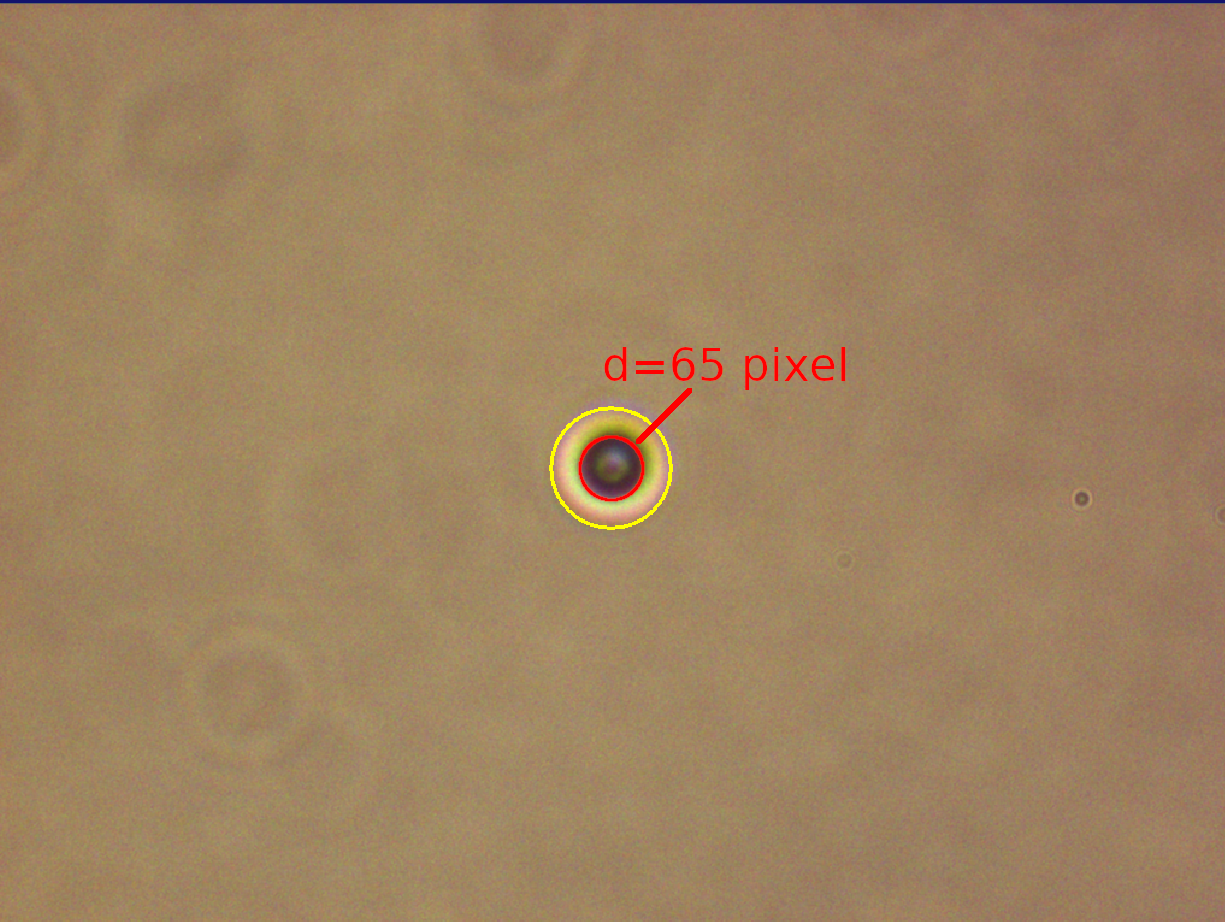
\includegraphics[width = 0.75\textwidth]{pictures/cal_cam.png}
            \caption{Abbildung der vier vermessenden Vesikel, die rot hervorgehoben und deren Größe in Pixeln angegeben sind.}
            \label{fig:cal_cam}
            \end{figure}
            \FloatBarrier
            %


        \subsubsection{Kalibrierung der Photodiode}
            Die zur Kalibrierung der Photodiode aufgenommenen S-Kurven sind exemplarisch für eine Laserleistung von \SI{4.83}{\milli\watt} in einem Screenshot des Programms \ref{fig:pos_cal} für die x- und 
            y-Achse dargestellt. In diesem Screenshot sind auch die per Programm berechneten und in Grafik \ref{fig:Konversion} gegen die Laserleistung aufgetragenen Konversionsfaktoren der beiden Achsen 
            eingetragen. Dabei ergibt sich ein linearer Abfall der Konversionsfaktoren, die zur Berechnung der Position eines eingefangenen Objekts durch die von der Vier-Segment-Diode gemessenen Spannung 
            benötigt wird.
            %
            \begin{figure}[h]
            \centering
            \includegraphics[width = 0.75\textwidth]{OP_Sternikov/Pos_Cal_50mA.png}
            \caption{Abbildung der vier vermessenden Vesikel, die rot hervorgehoben und deren Größe in Pixeln angegeben sind.}
            \label{fig:pos_cal}
            \end{figure}
            \FloatBarrier
            %         
            %
            \begin{figure}[h]
            \centering
            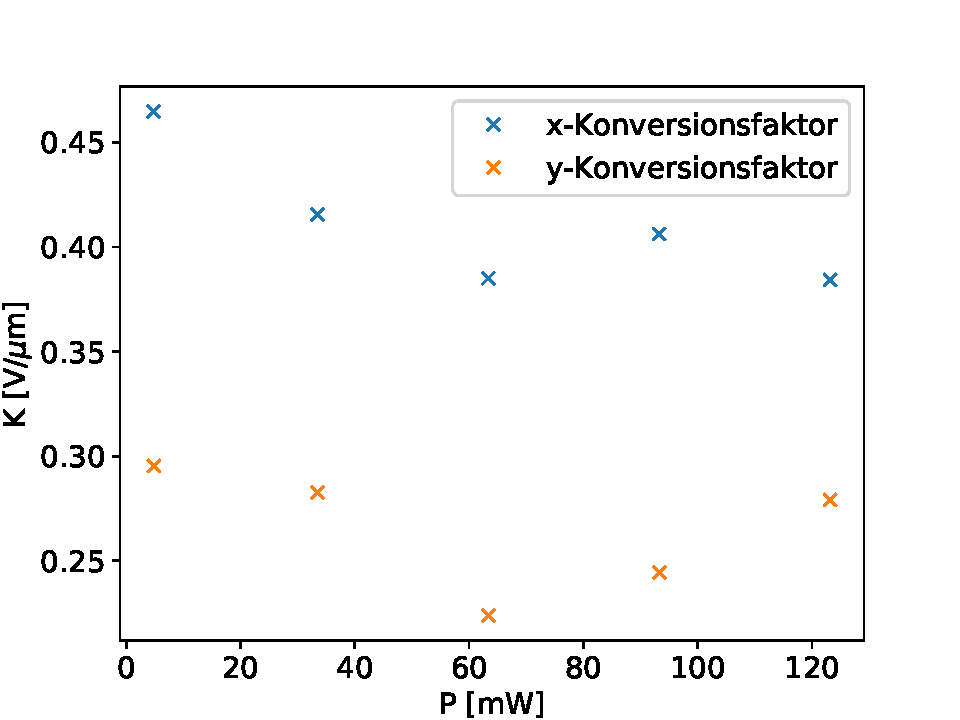
\includegraphics[width = 0.75\textwidth]{Konversion.pdf}
            \caption{Abbildung der vier vermessenden Vesikel, die rot hervorgehoben und deren Größe in Pixeln angegeben sind.}
            \label{fig:Konversion}
            \end{figure}
            \FloatBarrier
            %
            Das in Abhängigkeit des z-Piezo-Werts aufgenommene Diodensummensignal bei einem festen Quarzkügelchen ist in Abbildung \ref{fig:Diodensumme} aufgetragen. Der Verlauf der Kurve entspricht dem
            nach Abbildung REF ZU THEORIE zu erwartenden Anstiegt in der Umgebung des Streumaximus und bestätigt, dass ein festes Quarzkügelchen vermessen wurde.
            %
            \begin{figure}[h]
            \centering
            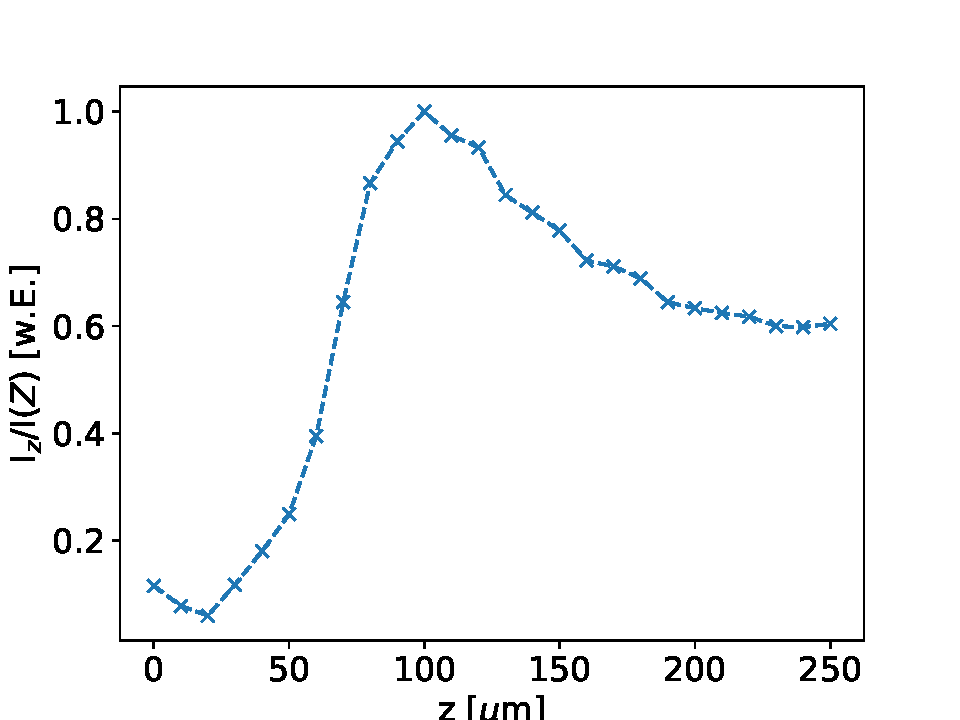
\includegraphics[width = 0.75\textwidth]{Diodensumme.pdf}
            \caption{Abbildung der vier vermessenden Vesikel, die rot hervorgehoben und deren Größe in Pixeln angegeben sind.}
            \label{fig:Diodensumme}
            \end{figure}
            \FloatBarrier
            %


            
        \subsubsection{Kalibrierung der Fallensteifigkeit}
            Der letzte Schritt der Kalibrierung, umfasst die Bestimmung der Fallensteifigkeiten $k_x$ und $k_y$ für beide Achsen.
            
            Für die Kalibrierung ohne externe Krafteinwirkung wird die spektrale Leistungsdichte (PSD) genutzt, die im Screenshot \ref{fig:PSD} für beide Achsen bei einer Laserleistung von 
            \SI{63.4}{\milli\ampere} dargestellt ist und direkt aus dem Programm exportiert werden kann. 
            %
            \begin{figure}[h]
            \centering
            \includegraphics[width = 0.75\textwidth]{OP_Sternikov/k_noForce_150mA.png}
            \caption{Abbildung der vier vermessenden Vesikel, die rot hervorgehoben und deren Größe in Pixeln angegeben sind.}
            \label{fig:PSD}
            \end{figure}
            \FloatBarrier
            %
            An diese Kurve wird folgende Funktion angepasst
            \begin{equation*}
                \text{PSD}(f) = \text{const} \cdot \frac{1}{f^2+f_0^2} \, ,
            \end{equation*}
            die die Frequenz $f$ sowie die sogenannte Roll-Off-Frequenz $f_0$ beinhaltet und die Eigenschaften der spektralen Leistungsdichte REF ZUR THEORIE wiedergibt. Aus diesen in Grafik 
            \ref{fig:freq_noForce} exemplarisch für eine Laserleistung von \SI{63.4}{\milli\ampere} dargestellten Anpassungen, werden die Fallensteifigkeiten über Formel REF ZUR THEORIE ausgerechnet und in Tabelle
            \ref{tab:noForce} aufgetragen. Da der erste und letzte Wert deutlich vom zu erwartenden ansteigenden Trend der drei mittleren Werte abweichen, wird nur durch diese drei mittleren Werte eine Ausgleichsgerade zur 
            Kalibrierung der Fallensteifigkeit in Abhängigkeit des Pumpstrom gelegt. Dies ergibt folgende Kalibrierung in Abhängigkeit der Laserleistung in \si{\milli\watt} für den Bereich 
            von \SI{93.3}{\milli\watt} bis \SI{153.1}{\milli\watt}:
            \begin{align}
                k_x(\text{P}) &= 1.34\cdot10^{-8}\si{\newton\per\metre\milli\watt} - 7.71\cdot10^{-7}\si{\newton\per\metre} \\
                k_y(\text{P}) &= 2.14\cdot10^{-8}\si{\newton\per\metre\milli\watt} - 1.46\cdot10^{-6}\si{\newton\per\metre}
            \end{align}
            %
            \begin{figure}[h]
            \centering
            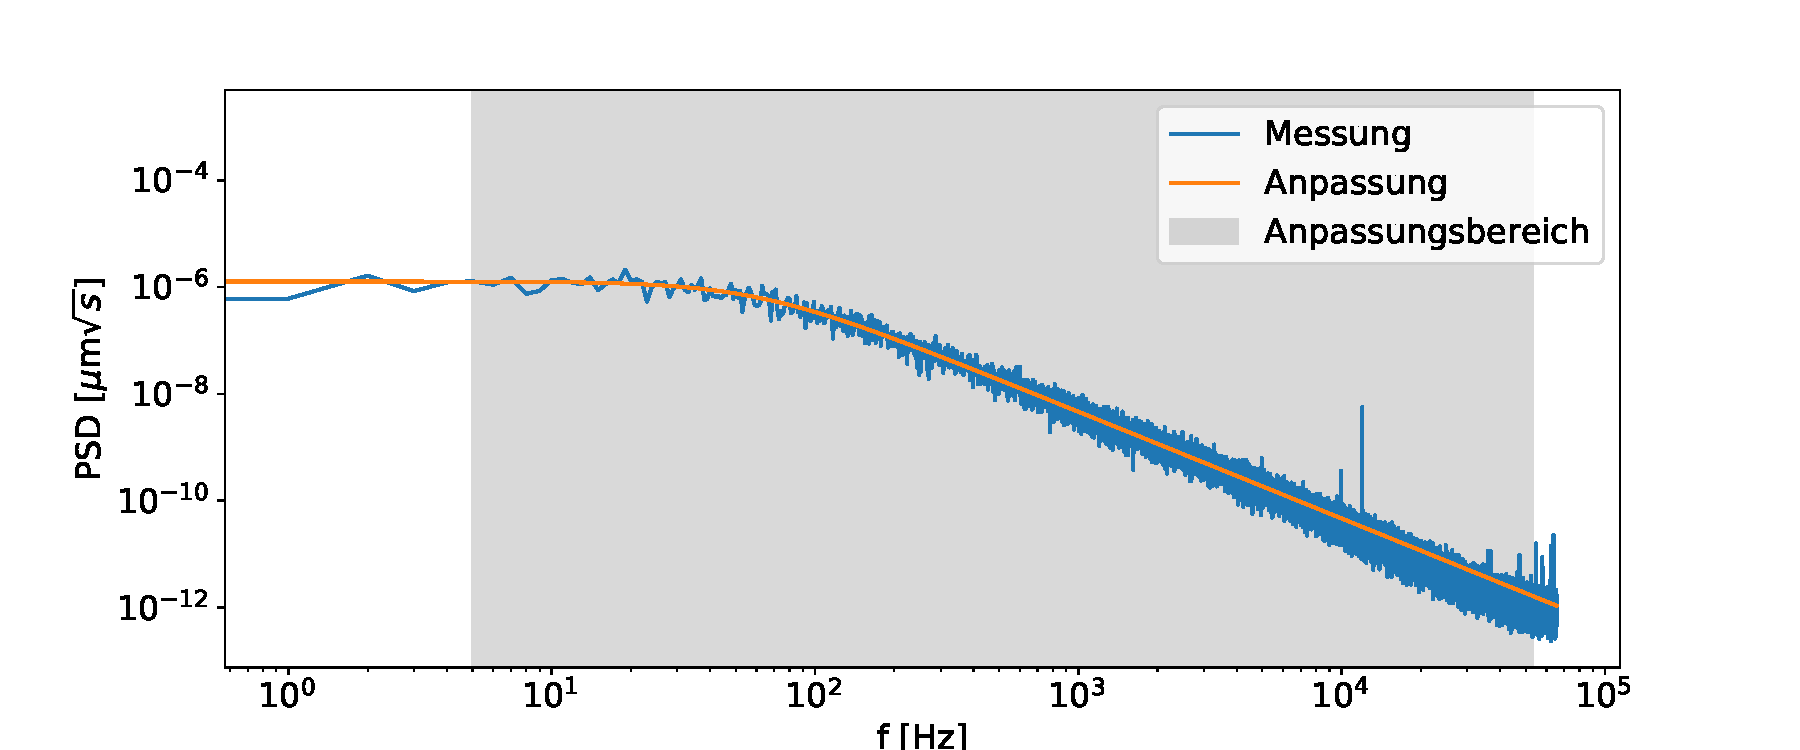
\includegraphics[width = 0.7\textwidth]{freq_x.pdf}
            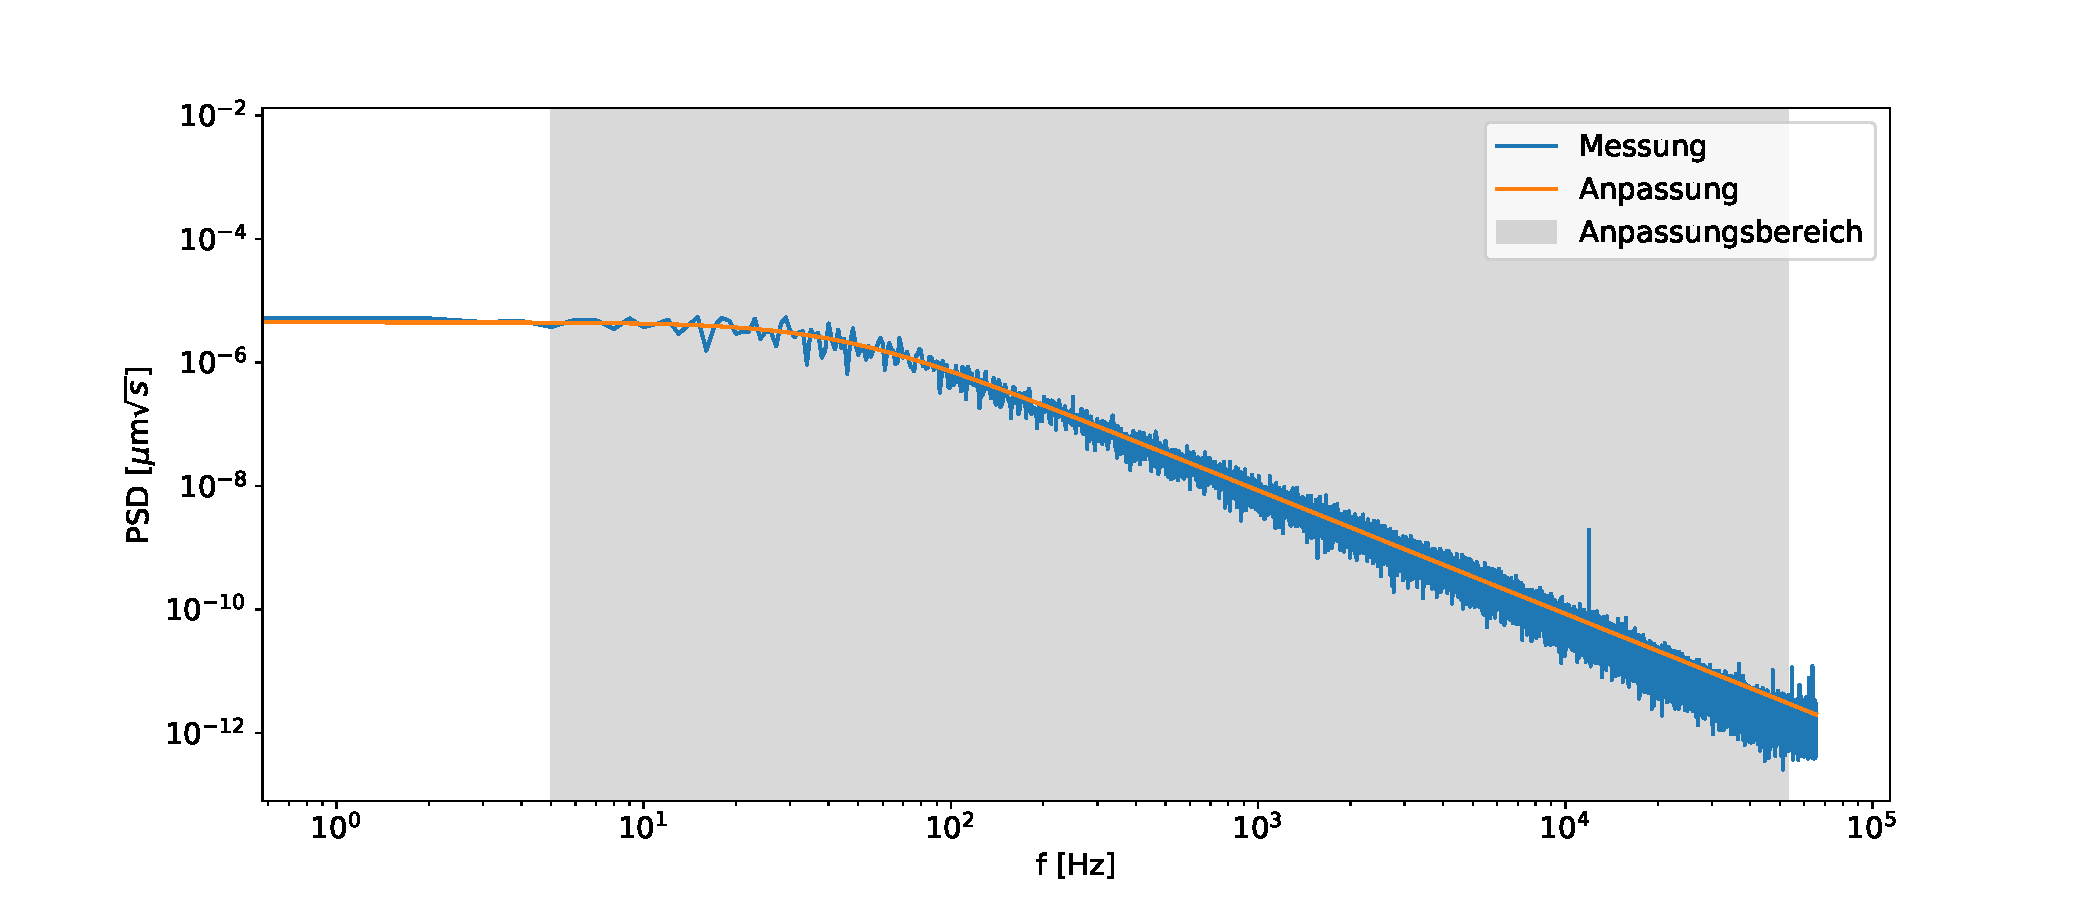
\includegraphics[width = 0.7\textwidth]{freq_y.pdf}
            \caption{Die spektrale Leistungsdichte gegen die Frequenz aufgetragen sowie eine theoretische Anpassungen, die auf den Werten im markierten Bereich beruht.}
            \label{fig:freq_noForce}
            \end{figure}
            \FloatBarrier
            % 
            %
            \begin{figure}[h]
            \centering
            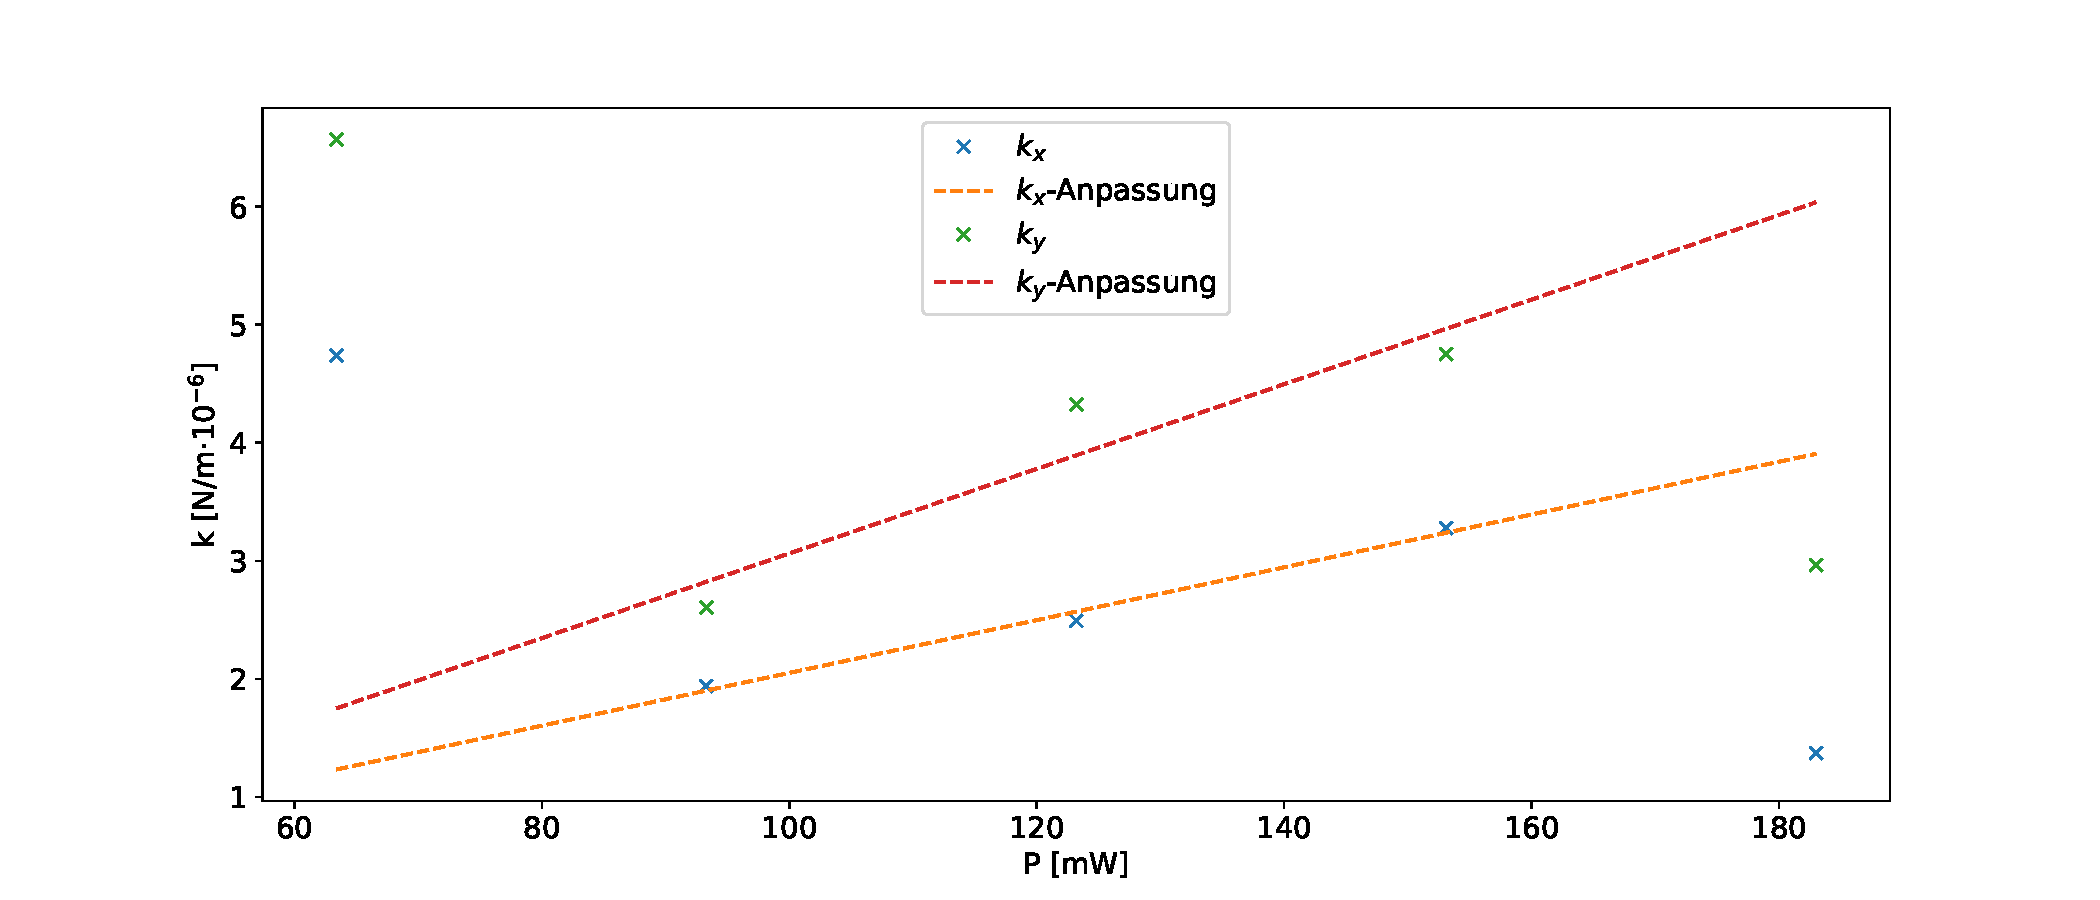
\includegraphics[width = 0.75\textwidth]{k_noForce.pdf}
            \caption{Aus den PSD-Anpassungen gewonnene Fallensteifigkeiten aufgetragen gegen die Laserleistung und eine lineare Anpassung der mittleren drei Werte zur Kalibrierung der Fallensteifigkeiten.}
            \label{fig:k_noForce}
            \end{figure}
            \FloatBarrier
            %
            Zur Überprüfung der Kalibrierung wird aus der Variation der Position des Kügelchens aufgrund der Brown´schen Bewegung, die in den Grafiken \ref{fig:pos_noForce} für eine Laserleistung von 
            \SI{63.4}{\milli\watt}
            dargestellt ist, und den zuvor berechneten Fallensteifigkeiten die Boltzmankonstante zu den in Tabelle \ref{tab:noForce} aufgelisteten Werten bestimmt.
            %
            \begin{table}[h]
                \centering
                \caption{Die Durchmesser der 4 vermessenen Vesikel in der Einheit von Pixeln und im Realraum}
                \label{tab:noForce}
                \begin{tabular}{c c c c c}
                \toprule
                {P[mW]} &   {$k_\text{x}$ [N/m]} & {$k_\text{B,x}$ [J/K]} &{$k_\text{y}$ [N/m]} & {$k_\text{B,y}$ [J/K]}  \\
                \midrule
                \num{63.4}     &   \num{4.74e-6}	 &  \num{2.42e-24}   &  \num{6.57e-6}    &  \num{1.34e-24}  \\
                \num{93.3}     &   \num{1.94e-6}	 &  \num{1.31e-24}   &  \num{2.61e-6}    &  \num{1.10e-24}  \\
                \num{123.2}    &   \num{2.49e-6}	 &  \num{1.32e-24}   &  \num{4.33e-6}    &  \num{1.35e-24}  \\
                \num{153.1}    &   \num{3.28e-6}	 &  \num{1.40e-24}   &  \num{4.75e-6}    &  \num{1.22e-24}  \\
                \num{182.0}    &   \num{1.37e-6}	 &  \num{1.13e-24}   &  \num{2.96e-6}    &  \num{7.53e-25}  \\
                \bottomrule
                \end{tabular}
            \end{table}
            %
            %
            \begin{figure}[h]
            \centering
            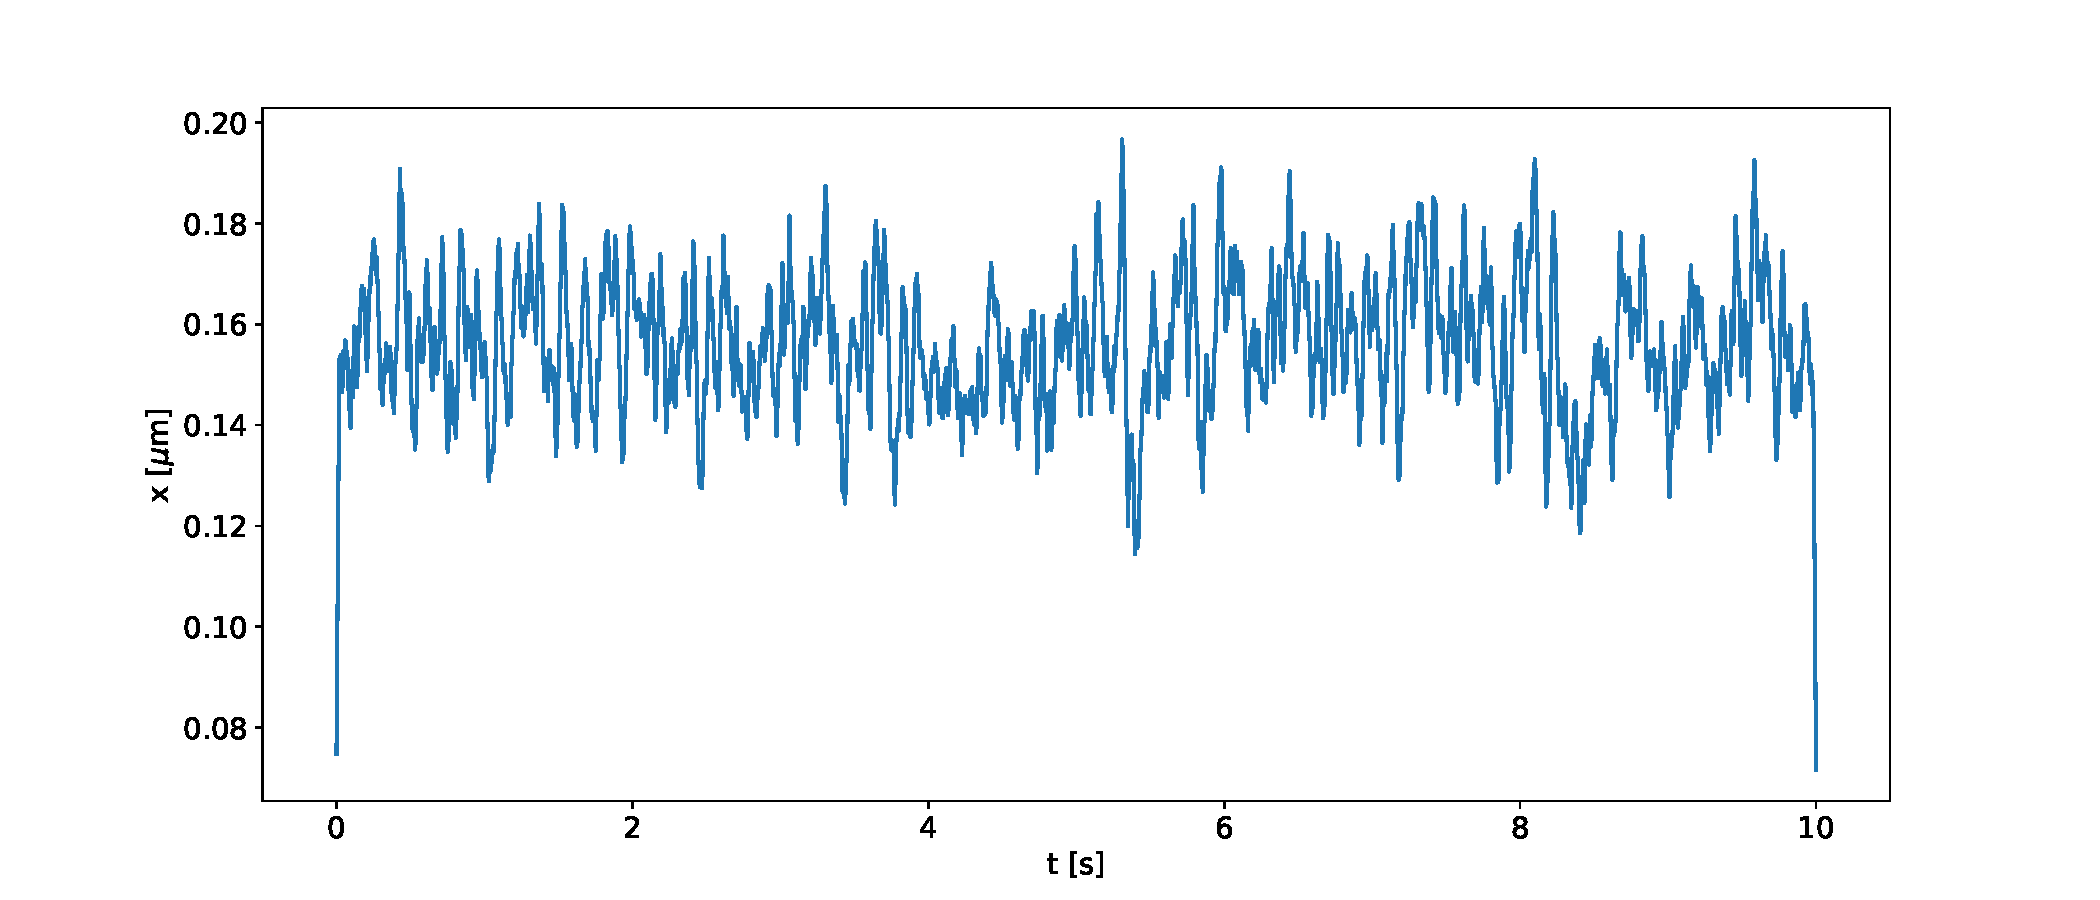
\includegraphics[width = 0.7\textwidth]{force_x.pdf}
            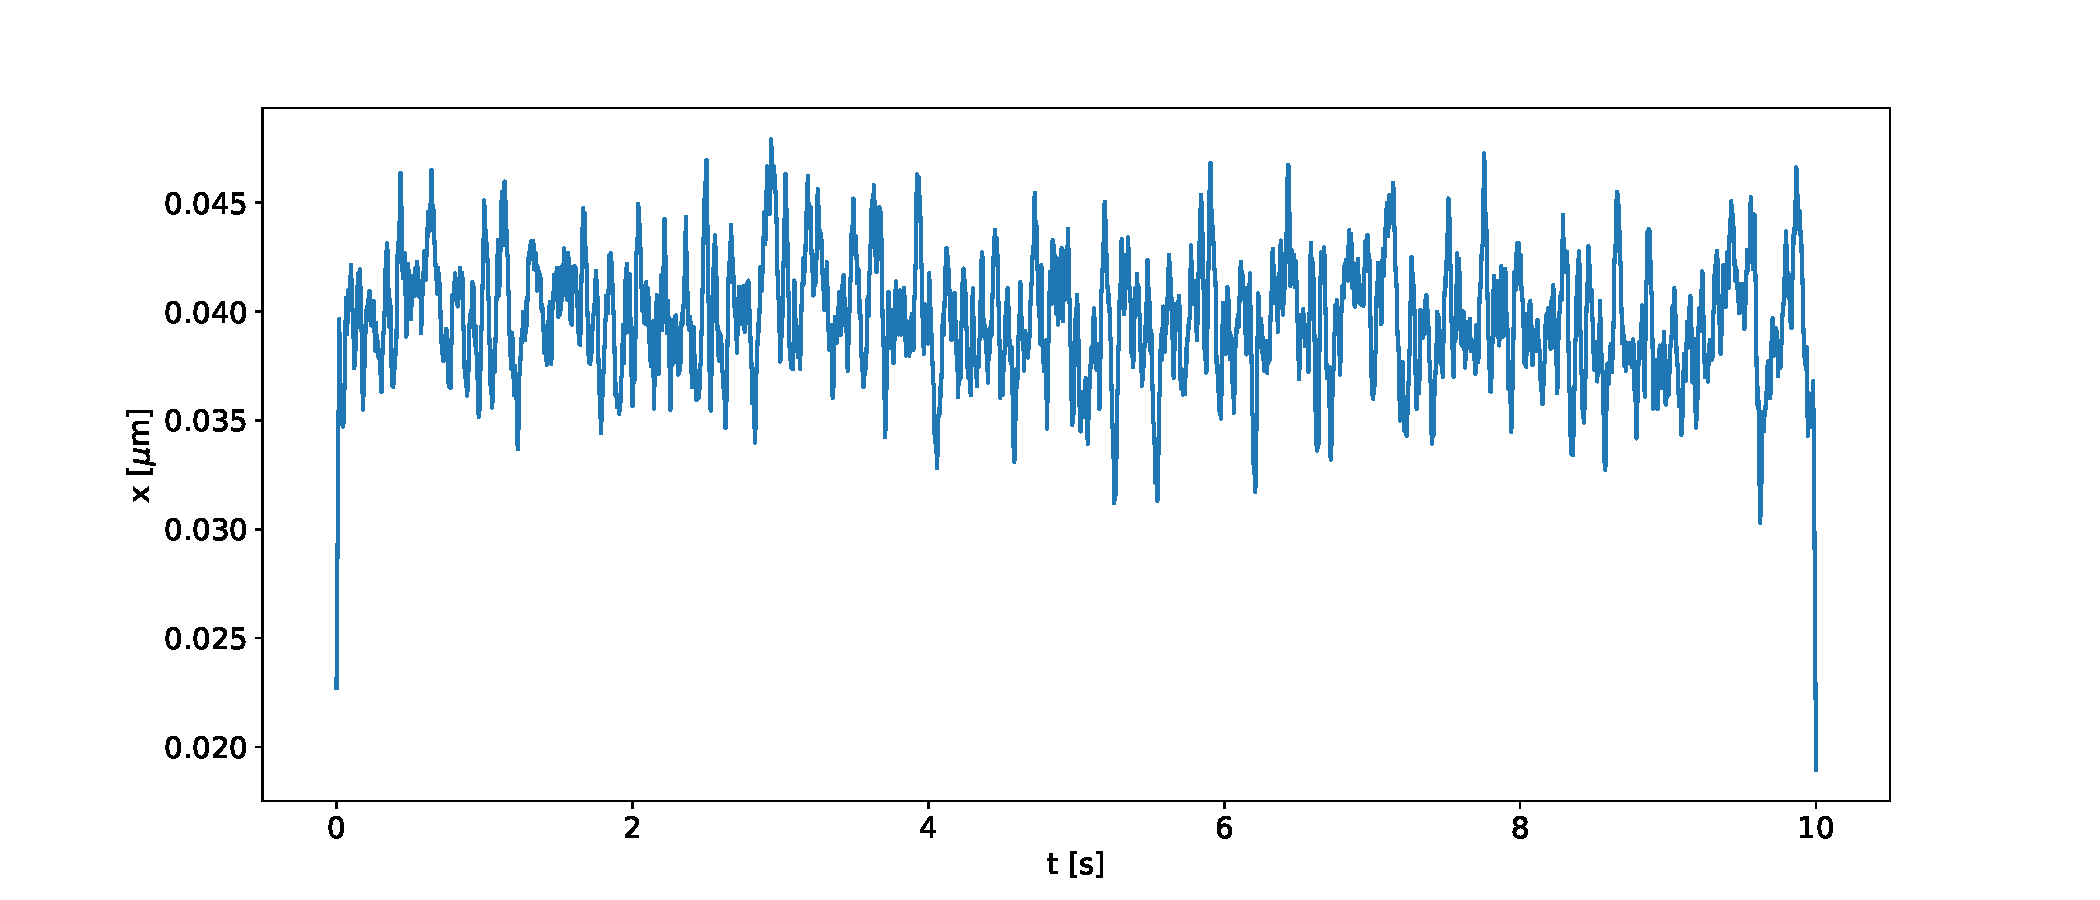
\includegraphics[width = 0.7\textwidth]{force_y.pdf}
            \caption{Der Ort des Quarzkügelchens aufgetragen gegen die Messzeit.}
            \label{fig:pos_noForce}
            \end{figure}
            \FloatBarrier
            % 

            
            Bei Anregung mit einer externen Kraft kann die Bewegung des Quarzkügelchens als sinusförmige Schwingung
            \begin{equation*}
                x(t) = \text{A} \sin\left(2\pift\right)
            \end{equation*}
            mit der Amplitude A und der Frequenz $f$ beschrieben werden. So lässt sich die wirkende Kraft mit Hilfe der Fallensteifigkeit $k_{x/y}$ berechnen. Wenn das Quarzkügelchens die optische Pinzette 
            aufgrund der externen Kraft verlässt, kann die dort wirkende Kraft mit dem zuvor beschriebenen Weg zur Kraftberechnung gleichgesetzt werden. Es ergibt sich folgende Gleichung
            \begin{equation*}
                da
            \end{equation*} 
            



    \newpage
    \subsection{Untersuchung des Vesikeltransports in Zwiebeln}
        \FloatBarrier
        Zur Charakterisierung der Vesikel werden zunächst die Größen der vier in Abbildung \ref{fig:vesikel_size} rot hervorgehobenen Vesikel bestimmt. Dazu wird der Durchmesser der Vesikel über eine 
        Bildbearbeitungssoftware in der Einheit pixel bestimmt und anschließend über die in Abschnitt REF berechnete Größe eines Pixels im Realraum zu den in Tabelle \ref{tab:d_vesikel} aufgelisteten Werten 
        umgerechnet. Im Mittel ergibt sich so ein Vesikeldurchmesser d$_\text{Vesikel}$ von \SI{0.705}{\micro\metre}.
        %
        \begin{table}[h]
            \centering
            \caption{Die Durchmesser der 4 vermessenen Vesikel in der Einheit von Pixeln und im Realraum}
            \label{tab:d_vesikel}
            \begin{tabular}{c c}
            \toprule
            {d$_\text{Vesikel}$ [Pixel]} & {d$_\text{Vesikel}$ [$\mu$m]}  \\
            \midrule
            21	 &  0.666  \\
            19	 &  0.602  \\
            21	 &  0.666  \\
            28	 &  0.887  \\
            \bottomrule
            \end{tabular}
        \end{table}
        %
        \begin{figure}[h]
        \centering
        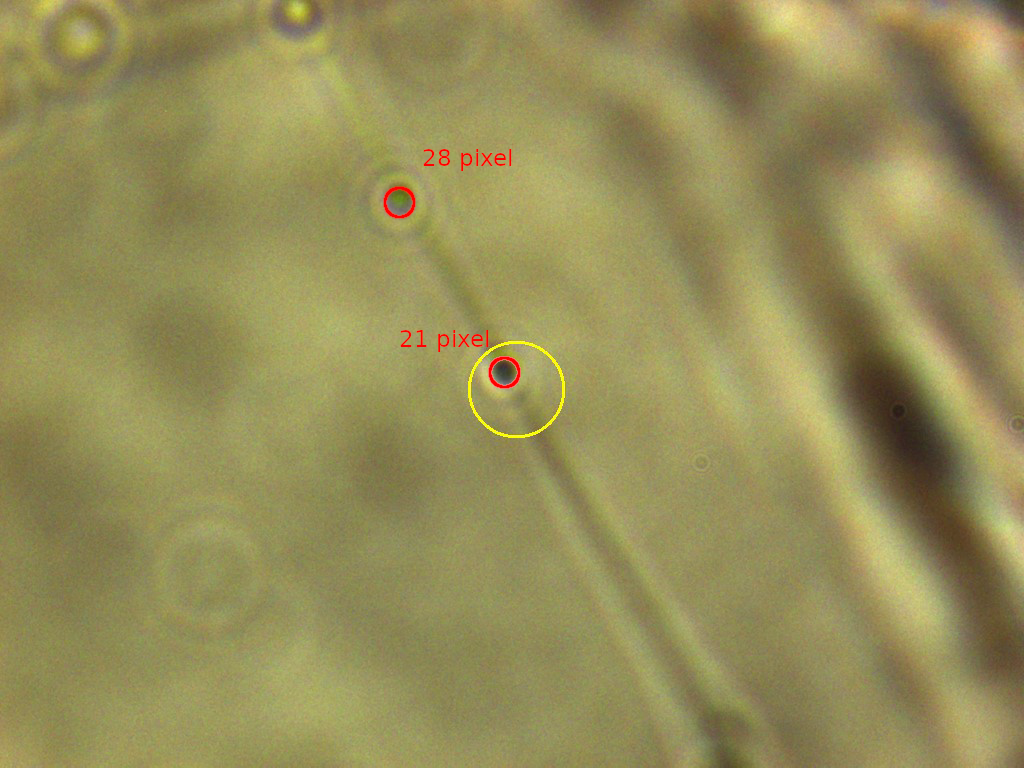
\includegraphics[width = 0.4\textwidth]{pictures/vesikel_size_1.png}
        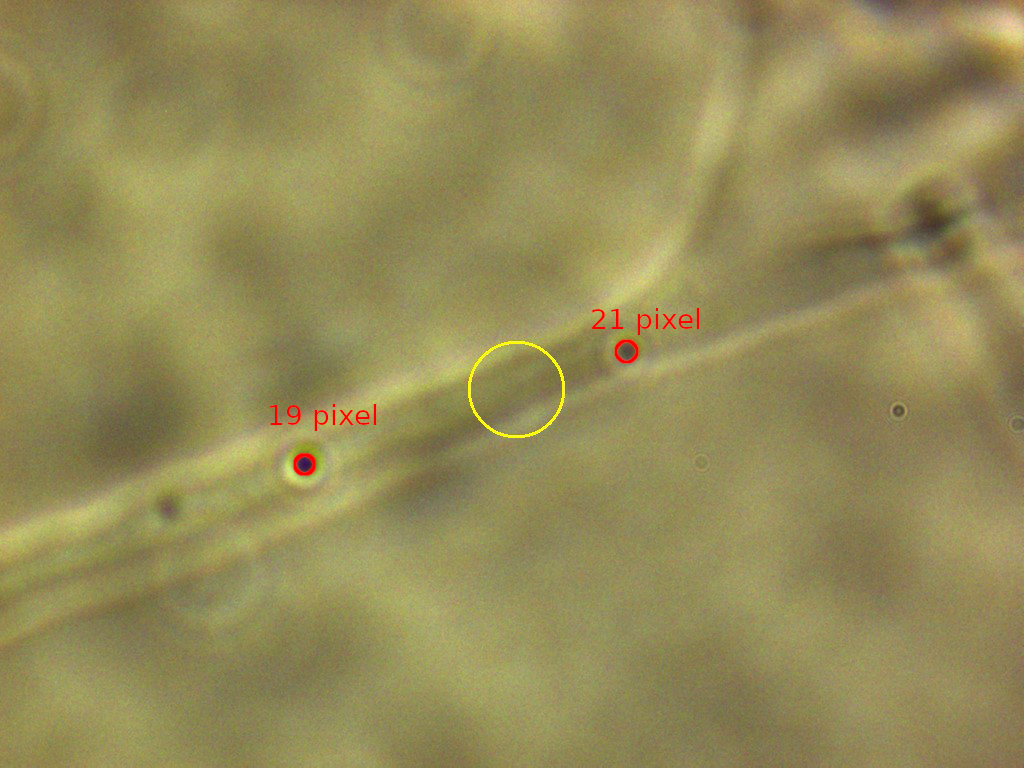
\includegraphics[width = 0.4\textwidth]{pictures/vesikel_size_2.png}
        \caption{Abbildung der vier vermessenden Vesikel, die rot hervorgehoben und deren Größe in Pixeln angegeben sind.}
        \label{fig:vesikel_size}
        \end{figure}

        \FloatBarrier
        %
        \newpage
        Zur Bestimmung der Geschwindigkeit des Vesikeltransports ist die Intensität der Photodiode gegen die Zeit beim Durchlauf eines Vesikels durch die optische Falle in Abbildung 
        \ref{fig:vesikel_size} aufgetragen. Daraus geht eine Durchquerungszeit $\Delta$t von \SI{1}{\second} hervor, die auf eine Vesikelgeschwindigkeit von 
        %
        \begin{equation*}
            v_{\text{Vesikel}} = \frac{2\text{d}_\text{Vesikel}}{\Delta\text{t}} = \SI{1.410}{\micro\metre\per\second}
        \end{equation*}
        %
        schließen lässt.
        %
        \FloatBarrier
        %
        \begin{figure}[h]
        \centering
        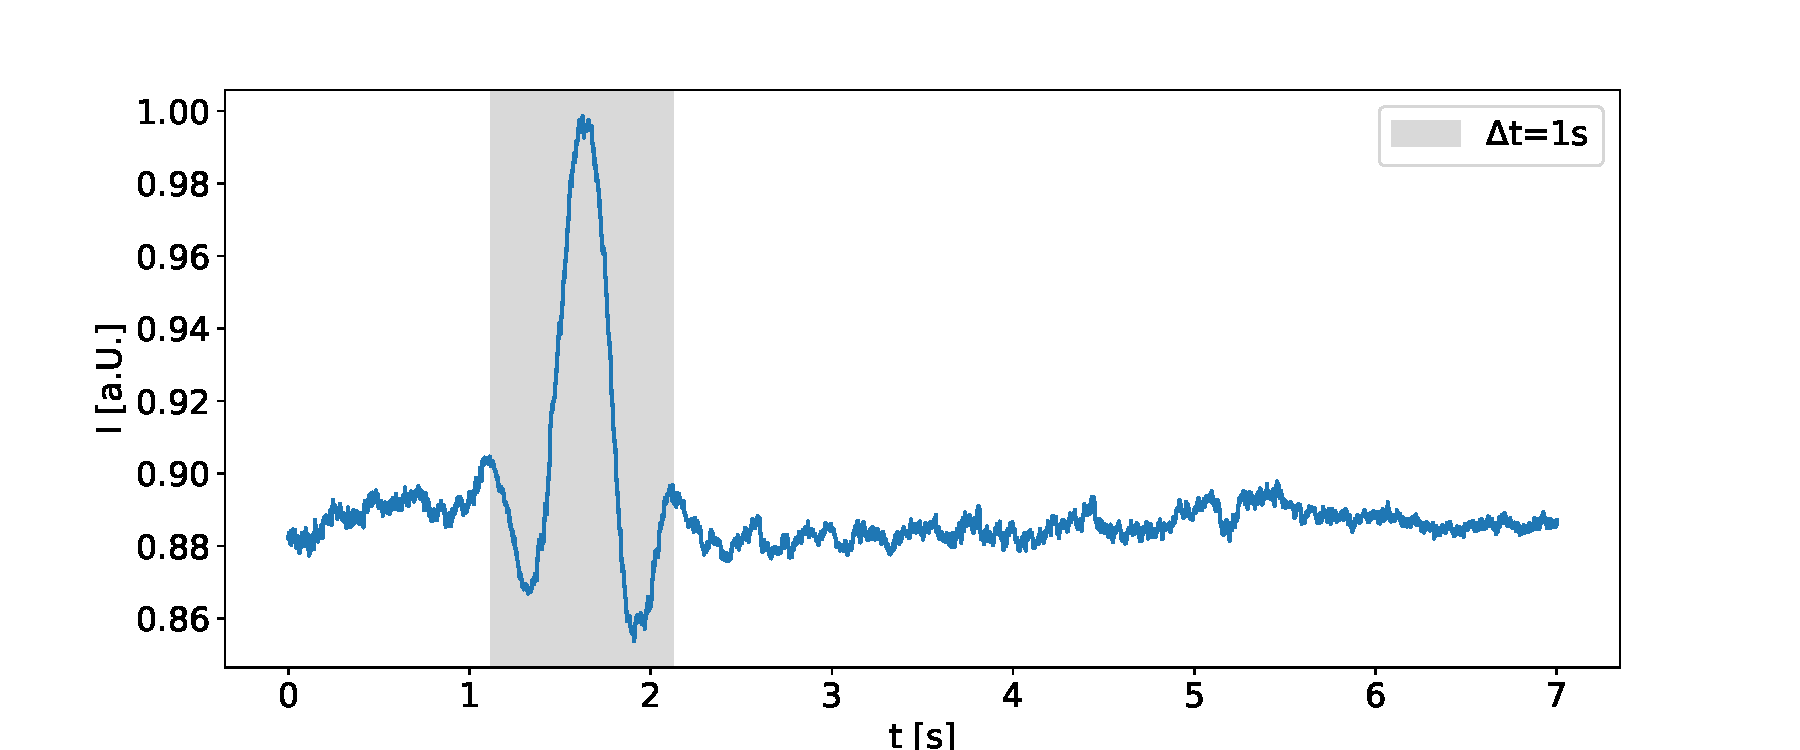
\includegraphics[width = 0.8\textwidth]{v_vesikel.pdf}
        \caption{Auf die Dauer einer Sekunde bestimmte Intensitätsänderung aufgrund des Durchlaufens eines Vesikels durch die optische Falle.}
        \label{fig:v_vesikel}
        \end{figure}
        %
        \FloatBarrier
        %
        \newpage
        Aus den restlichen Videoaufnahmen lassen sich weitere Schlüssel über das typische Verhalten des Vesikeltransports ziehen. So laufen entlang einer Actin-"Straße" alle Vesikel entlang einer Richtung
        und überholen sich nicht. Wenn ein Vesikel mit Hilfe der optischen Pinzette gegriffen wird, kann es, wie in Abbildung \ref{fig:vesikel_abstand} zu sehen, über \SI{16}{\micro\metre} weit von der 
        Actin-"Straße" entfernt werden, ohne dass sich die Bindung der Myosin-Motoren zwischen der Straße und dem Vesikel lösen. Bei Deaktivieren der optischen Pinzette springt das Vesikel zunächst zurück 
        an seine alte Position und läuft dann weiter in die ursprüngliche Richtung. 
        %
        \FloatBarrier
        %
        \begin{figure}[h]
        \centering
        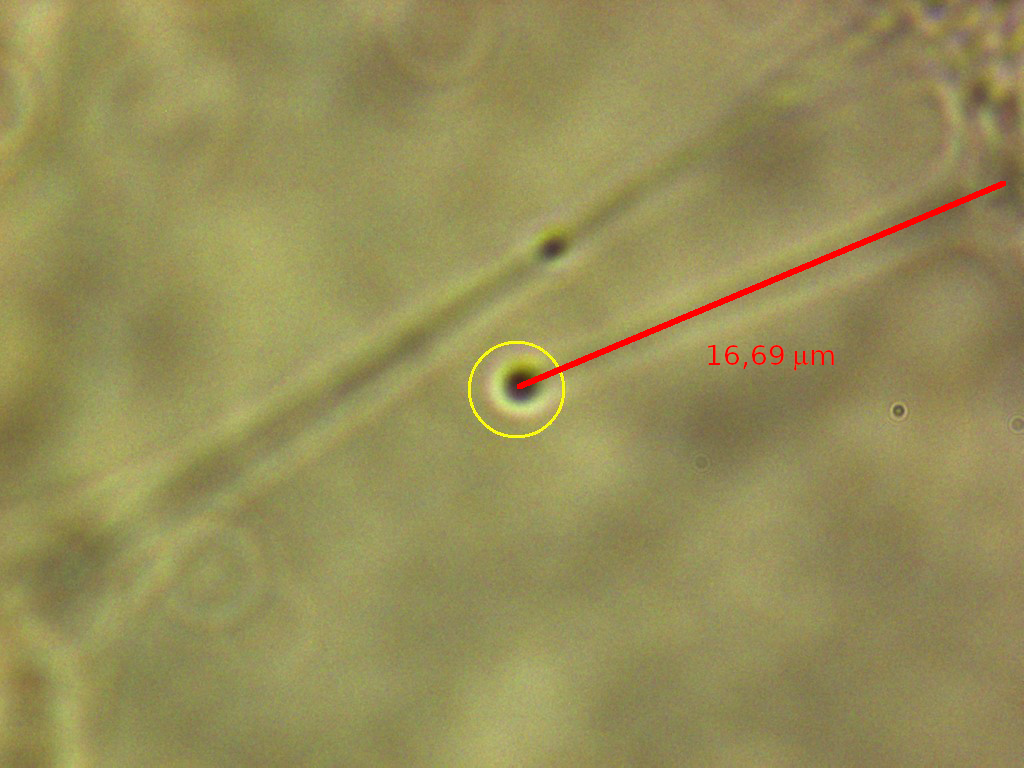
\includegraphics[width = 0.4\textwidth]{pictures/vesikel_abstand.png}
        \caption{Ein Vesikel, das über \SI{16}{\micro\metre} von seiner Ausgangsposition auf der Actin-Straße entfernt wurde.}
        \label{fig:vesikel_abstand}
        \end{figure}
        %
        \FloatBarrier 
        %
        Da die Verbindung der Myosin-Motoren nicht gebrochen werden kann, war es auch nicht möglich Vesikel von einer Straße durch Bereiche ohne Straße auf eine andere zu transferieren. Dies ist in Abbildung
        \ref{fig:vesikel_overlap} zu sehen. Ein Vesikel wird von der Straße am rechten Ende der roten Linie abgefangen und direkt über der blauen Straße platziert. Beim Deaktivieren der optischen Falle geht das 
        Vesikel auf seine Ausgangsposition auf der ehemaligen Straße zurück. 
        %
        \FloatBarrier
        %
        \begin{figure}[h]
        \centering
        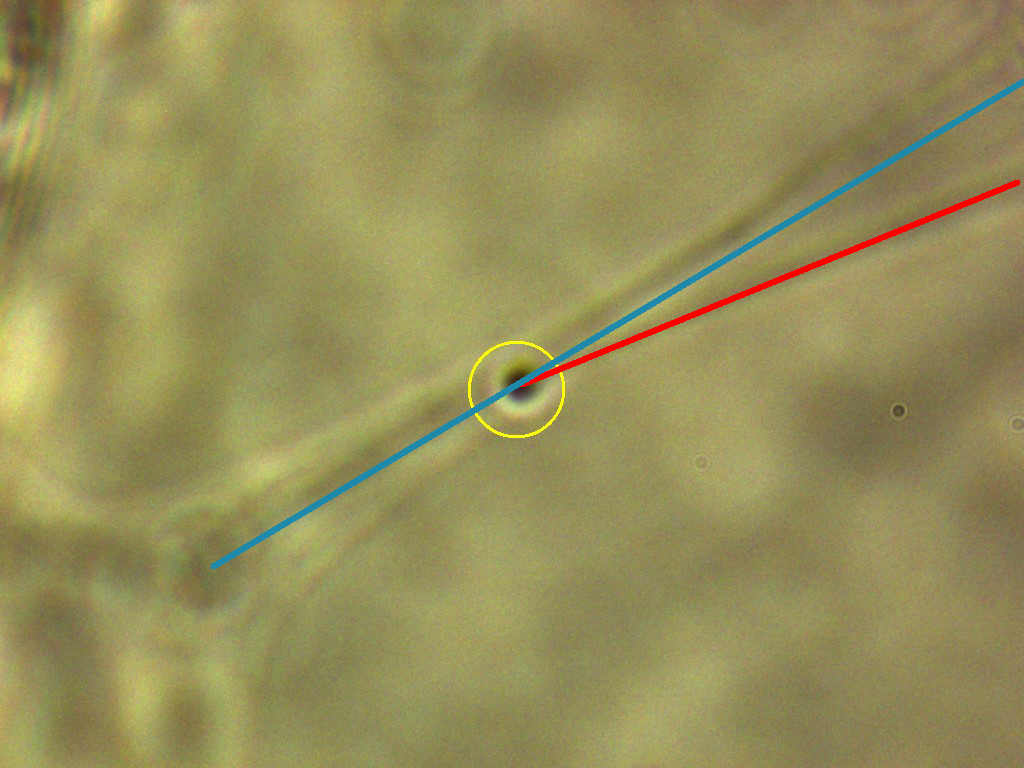
\includegraphics[width = 0.4\textwidth]{pictures/vesikel_overlap.png}
        \caption{Das über der blauen Straße platzierte Vesikel springt bei Deaktivierung der optische Falle auf seine Ausgangsposition auf der Straße am rechten Ende der roten Linie zurück.}
        \label{fig:vesikel_overlap}
        \end{figure}
        %
        \FloatBarrier 
        %
        \newpage
        Auch beim Entfernen der Vesikel von der Straße sind diese jedoch noch beweglich, da die Myosin-Motoren weiterhin funktionieren. In der Nähe einer Kreuzung ist so das schnelle verschieben der 
        Myosin-Motoren entlang der Kreuzung durch Verschieben des Vesikels, wie in Abbildung \ref{fig:vesikel_sprung} schematisch eingezeichnet, möglich.
        %
        \FloatBarrier
        %
        \begin{figure}[h]
        \centering
        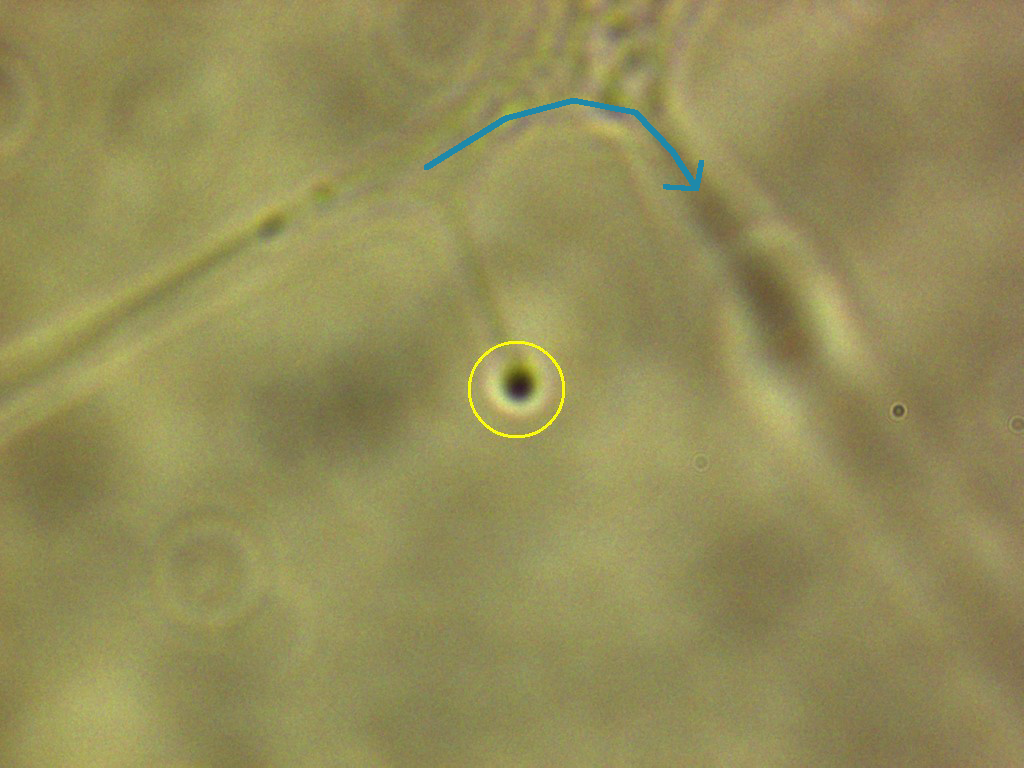
\includegraphics[width = 0.4\textwidth]{pictures/vesikel_transport.png}
        \caption{Bei der gegebenen Vesikelposition können die Myosin-Motoren entlang der Kreuzung auf die andere Straße verfahren.}
        \label{fig:vesikel_sprung}
        \end{figure}
        %
        \FloatBarrier 
        %
        Durch Platzierung der optischen Pinzette über einer Actin-Straße und sukzessivem Erhöhen der Laserleistung ist ein Stopp des Vesikeltransports bei einer Laserleistung von \SI{63}{\milli\watt} zu 
        beobachten. Dies entspricht einer aufgrund der schlechten Kalibrierungsmessungen nur abzuschätzenden Fallensteifigkeit von einigen wenigen \SI{10e-6}{\newton\per\metre}. 